
\section{Problem Formulation}
\label{sec:problemformulation}

Assume that the target space is discretized into $J$ locations. 
This can be of any level of granularity 
depending on the desired accuracy. Finer granularity does increase computational load, but does not seem to be a bottleneck. There are a set of sniffers or APs doubling as sniffers (a larger number is expected to improve accuracy) that report a vector of RSSs from a target device to be localized to a server that performs the necessary computation. The target device can be static or mobile. In fact, mobility tends to improve performance (more on this later). The location of the sniffers themselves are assumed to be known with respect to which the $J$ locations
are specified. No prior wireless measurements are needed, providing our approach with a significant leverage. 

\subsection{Using Gaussian Mixture Model}
We use the well-known idea of {\em mixture models} in statistics. The idea is to first make a very general assumption that the target could be in any of the $J$ possible locations with varying probabilities. Each of these possibilities can potentially generate a distribution of RSSs
at the set of sniffers. Now, given the vector of RSSs sniffed at the set of sniffers, the problem is to estimate the most likely target 
location out of the $J$ possibilities that could have generated that vector of RSSs. Since 
the same device at the same location but with a different transmit power can generate different distributions of RSSs, an additional subtlety we handle is that the
most likely power level (actually an abstract sense of it) is also
determined as a part of the process. This subtle addition makes the
method adaptive for different devices having their own default power
levels for wireless transmission.

\begin{figure} 
\centering
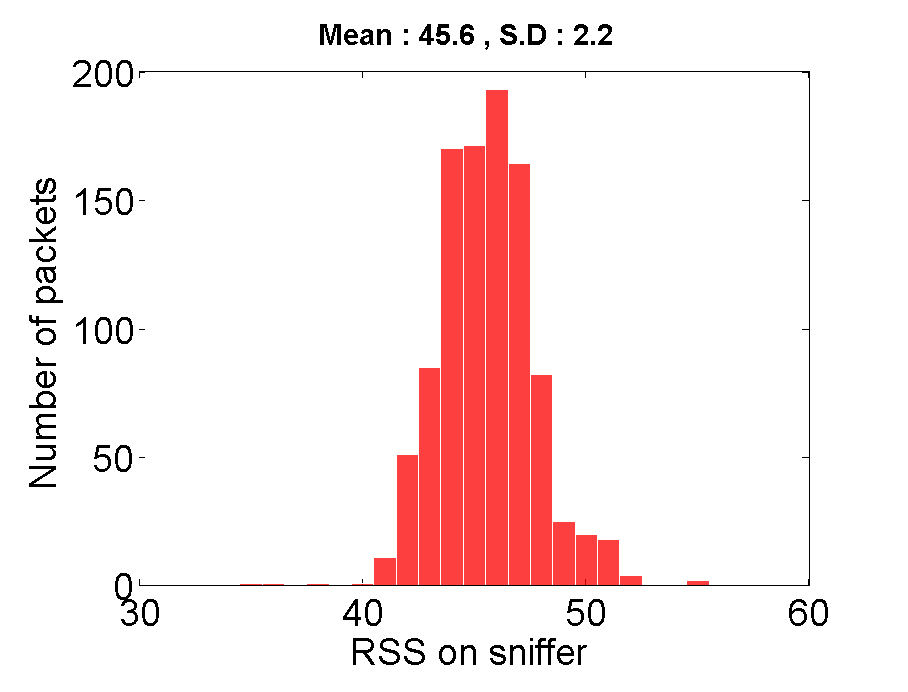
\epsfig{file=Figs4Paper/NewGaussian/distr7.eps, height=1.25in, width=1.6in} 
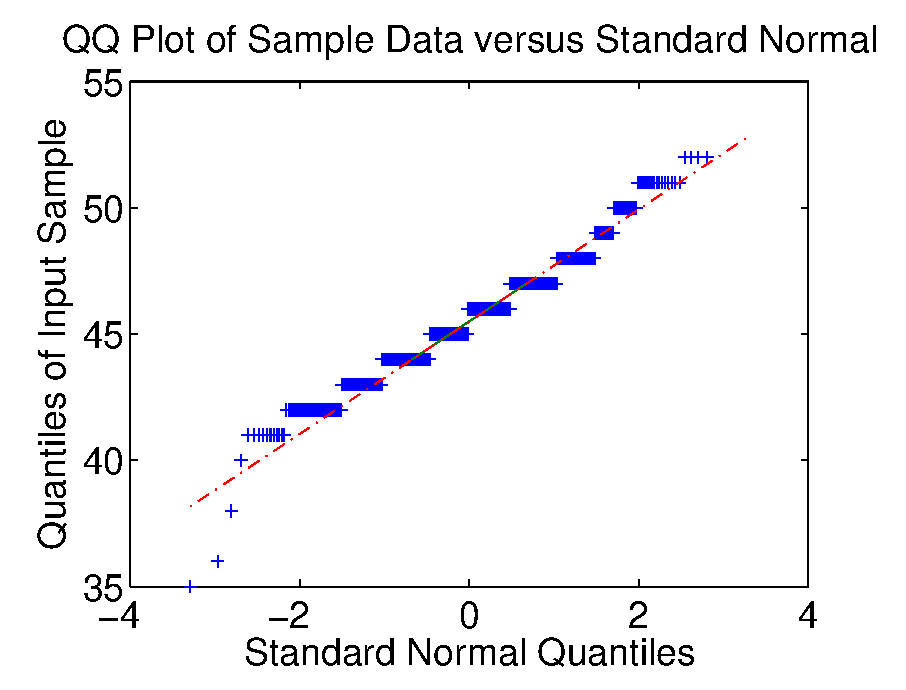
\epsfig{file=Figs4Paper/NewGaussian/qqplot2.eps, height=1.25in, width=1.6in}
\caption{The distribution of RSS observed on a sniffer.}
\label{fig:distribution}
\end{figure}

Before a more formal presentation, a key assumption we must make upfront
is that the distribution of RSS at a sniffer (more specifically an indicator representing RSS, commonly known as RSSI) is Gaussian
given the target device is stationary at a location and transmitting at
a fixed power level. The Gaussian assumption is not uncommon in wireless link modeling~\cite{Haeberlen:2004:PRL:1023720.1023728, Moraes:2006:CWL:1164783.1164799, Tao:2003:WLL:941311.941314}. In fact, the log-normal shadowing model~\cite{Rappaport:2001:WCP:559977} is widely used albeit in a slightly different context. To lend confidence to this assumption on our specific hardware setup, we have performed a set of measurements using the same sniffer and target device hardware used in later experiments. 
Figure~\ref{fig:distribution} shows the measured
RSSI distribution observed on a sniffer in our testbed 
for a stationary client transmitting at a fixed power level. The quality of the Gaussian fit for this distribution is also shown. The fit is very good. 

The Gaussian assumption makes our approach amenable to well-known machine learning tools. Now,
the distribution of the RSSs on the sniffers can be represented by the \emph{Gaussian Mixture Model} or GMM~\cite{Reynolds, Bishop:2006:PRM:1162264} --  a simple linear superposition of Gaussian components. 
Nothing is known a priori about the nature of these Gaussian
and in what proportion they are mixed. They are modeled in terms of discrete latent variables. We describe the modeling approach below.  

\subsection{Latent Variables for Target Locations and Power Levels}
\label{subsec:latentvariablesfortargetlocationsandpowerlevels}

Assume that a $J$-dimensional binary random variable {\bf x} representing possible target locations. $\mathbf{x}$ has a 1-of-$J$ representation in which a particular element $x_{j}$ is equal to one and all other elements are equal to $0$. The values of $x_{j}$ therefore satisfy $x_{j} \in$ \{0,1\} and $\sum_{j} x_{j} = 1$. Thus, there are $J$ possible states for the vector $\mathbf{x}$.

The probability distribution over $\mathbf{x}$ can be specified as a multinomial 
\begin{align}
 p(x_{j} = 1) = \upsilon_{j},
\end{align}
where the parameters $\{\upsilon_{j}\}$ must satisfy
\begin{align}
0 \le \upsilon_{j} \le 1 \ \text{and} \ \sum_{j=0}^{J} \upsilon_{j} = 1.
\end{align}

Similarly, assume that a $K$-dimensional binary random variable $\mathbf{z}$ representing Power Levels. $\mathbf{z}$ has a 1-of-$K$ representation in which a particular element $z_{k}$ is equal to 1 and all other elements are equal to 0. The values of $z_{k}$ therefore satisfy $z_{k} \in$ \{0,1\} and $\sum_{k} z_{k} = 1$. Vector {\bf z} has $K$ possible states.

The distribution over $\mathbf{z}$ is specified as a multinomial 
\begin{align}
p(z_{k} = 1) = \tau_{k},
\end{align}
where the parameters $\{\tau_{k}\}$ must satisfy
\begin{align}
0 \le \tau_{k} \le 1 \ \text{and} \  \sum_{k=0}^{K} \tau_{k} = 1.
\end{align}


\begin{figure} [h!]
\centering
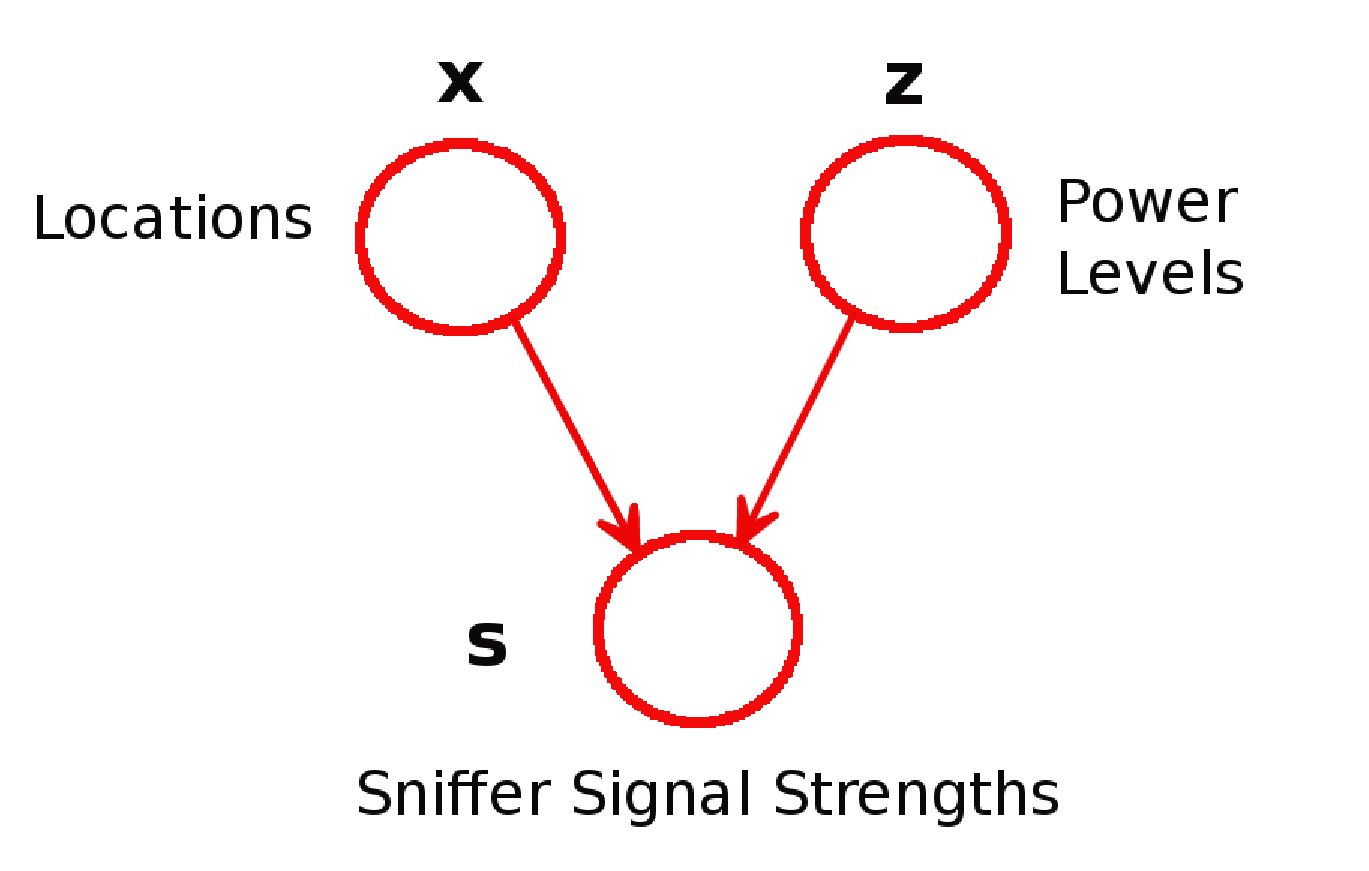
\epsfig{file=Figs4Paper/GMM/gmm4.eps, height=1.5in, width=2.5in}
\caption{The GMM for our problem.}
\label{fig:gmm}
\end{figure}


\subsection{RSSI Distribution}
\label{subsec:constructingthedistributionovertheobservedsignalstrengths}

Let $\mathbf{s}$ be the $N$-dimensional vector representing the RSSI observed by the $N$ sniffers in the target area. 
Using the chain rule of probability, we can now define the joint distribution $p(\mathbf{s}, \mathbf{x},\mathbf{z})$ in terms of the distribution $p(\mathbf{x},\mathbf{z})$ and the conditional distribution $p( {\bf s} | {\bf x}, {\bf z})$, 
corresponding to the graphical model in Figure \ref{fig:gmm}:
\begin{align}
p( {\bf s}, {\bf x}, {\bf z}) &= p( {\bf x}, {\bf z}) p( {\bf s} | {\bf x}, {\bf z}).
\end{align}
Since {\bf x} and {\bf z} are independent random variables,
\begin{align}
p( {\bf s}, {\bf x}, {\bf z}) &= p( {\bf x}, {\bf z}) p( {\bf s} | {\bf x}, {\bf z}) \nonumber \\
&= p({\bf x})p({\bf z})p( {\bf s} | {\bf x}, {\bf z}). \label{eqn:joint_distribution}
\end{align}

Equation \ref{eqn:joint_distribution} gives us the joint distribution of $ p( {\bf s}, {\bf x}, {\bf z}) $. The marginal distribution of {\bf s} is then obtained by summing the joint distribution over all possible states of {\bf x} and {\bf z}:
\begin{align}
p( {\bf s}) & = \sum_{\bf x}\sum_{\bf z} p({\bf x})p({\bf z})p({\bf s}|{\bf x}, {\bf z}).\label{eqn:marginal_distribution1}
\end{align}

%\subsubsection{Independence of Sniffers}
%\label{subsubsec:independenceofsniffers}

Now assume that the RSSIs observed at different sniffers are independent. This is justified as the sniffers are typically at disparate locations and thus the wireless propagation path loss can be assumed independent. 
Thus, the term $p( {\bf s} | {\bf x}, {\bf z})$ in equation
\ref{eqn:marginal_distribution1} can be simplified as
\begin{align}
p( {\bf s} | {\bf x}, {\bf z}) & = \prod_{i=1}^N p({s_{i}} | {\bf x}, {\bf
		z}). \label{eqn:conditional_distribution1}
\end{align}
Based on the Gaussian assumption made before, the RSSI can be modeled 
as Gaussian random variables determined by the (location, power-level) pair, so that
\begin{align}
s_{i} | {x_{j}=1}, {z_{k}=1}  \sim  \text{Gaussian}(\mu_{i, (j,k)}, \sigma_{i, (j,k)}).
\end{align}
This lends simplicity to our model since the term $p( {\bf s} | {\bf x}, {\bf z})$ in equation
\ref{eqn:conditional_distribution1} can be expressed succinctly as 
\begin{align}
p( {\bf s} | {\bf x}, {\bf z}) & =  \prod_{j=1}^J \prod_{k=1}^K 
		\prod_{i=1}^N \mathcal{N}(s_{i} |  \mu_{i, (j,k))},\sigma_{i, (j,k)}^2)^{x_j z_k} \, . \label{eqn:conditional_distribution2}
\end{align}
Note that for any given ${\bf x}$ and ${\bf z}$ only one term in the product is actually active for all $i$, because the exponent $x_j z_k$ acts as a selector: $x_j z_k = 1$ for exactly one index pair $(j,k)$, and equals $0$ for all others.

From now on, for notational convenience we define
\[
\mathcal{N}(\mathbf{s} |  \boldsymbol\mu_{(j,k))},\boldsymbol\sigma_{(j,k)}^2) \equiv \prod_{i=1}^N \mathcal{N}(s_{i} |  \mu_{i, (j,k))},\sigma_{i, (j,k)}^2) \, . 
\]

\subsection{Model Parameters}
\label{subsec:modelparameters}

Putting equations \ref{eqn:marginal_distribution1} and
\ref{eqn:conditional_distribution2} together we get the marginal probability distribution over
{\bf s} as
\begin{align}
p( {\bf s}) &= \sum_{j=1}^J \sum_{k=1}^K \upsilon_{j} \tau_{k} \mathcal{N}(\mathbf{s} |  \boldsymbol\mu_{(j,k))},\boldsymbol\sigma_{(j,k)}^2) \, .
\end{align}

Thus we have modeled the marginal distribution of {\bf s} as a Gaussian
mixture with target locations and power levels as the latent variables. The parameters of the model are 
\begin{align}
{\boldsymbol\theta} = \left( {\boldsymbol\upsilon} , {\boldsymbol\tau},  {\boldsymbol\mu} , {\boldsymbol\sigma}^2\right)\, .
\end{align}

Henceforth, we refer to this model as {\bf WiGMM}. We now use the widely popular \emph{Expectation-Maximization} (EM) algorithm~\cite{Dempster77maximumlikelihood, Borman_theexpectation, Bilmes97agentle, DinovIvoD, Bishop:2006:PRM:1162264} to estimate the parameters of the model.
